We have used our approach to model the decision process applied in the Apache project (the choice of Apache was motivated by the fact that it has a more complex governance process than other analyzed projects). 

We first represent the governance rules used to select tasks to accomplish. As described before, there are two types of voting procedures depending on whether the task to accomplish involves source code changes or not. The DSL defining the Apache governance rules is listed in Figure \ref{fig:rulesApache}.

\begin{figure}[t]
  \centering
  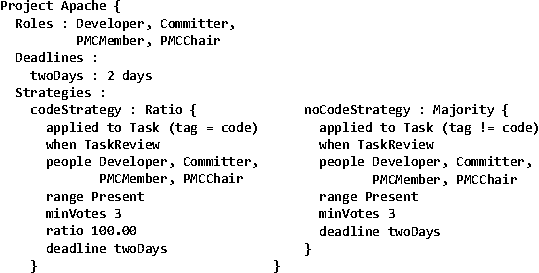
\includegraphics[width=0.65\textwidth]{./figures/apache}
  \caption{Apache governance rules.}
  \label{fig:rulesApache}
\end{figure}


%{\scriptsize
%\begin{verbatim}
%Project Apache {
%  Roles : Developer, Committer,
%          PMCMember, PMCChair
%  Deadlines :
%    twoDays : 2 days 
%  Strategies :
%    codeStrategy : Ratio { 
%      applied to Task (tag = code)
%      when TaskReview
%      people Developer, Committer, 
%             PMCMember, PMCChair
%      range Present
%      minVotes 3 
%      ratio 100.00 
%      deadline twoDays 
%    }, 
%    noCodeStrategy : Majority {
%      applied to Task (tag != code)
%      when TaskReview
%      people Developer, Committer, 
%             PMCMember, PMCChair
%      range Present
%      minVotes 3  
%      deadline twoDays
%    }
%}
%\end{verbatim}
%}

The example defines four roles and two strategies called \texttt{codeStrategy} and \texttt{noCodeStrategy}. The former is a ratio majority strategy which is applied to those tasks including the tag \texttt{code} (i.e., tasks involving changes in the code). All people belonging to the roles linked to the strategy (see tag \texttt{people}) and presently available (see tag \texttt{range}) can vote. It is required a ratio of agreement of 100\% (i.e., meaning that everybody has to agree) and at least three votes. Finally, the strategy defines a deadline of two days, although the precise length is not specified in the project documentation. On the other hand, \texttt{noCodeStrategy} is a majority strategy which is applied to those tasks not including the tag \texttt{code}. Like the previous strategy, it is required at least three votes to make a decision and the deadline is two days after the creation of the task. 

As an example of applying the previous rules, Figure \ref{fig:exampleCollaborationApache} shows a possible collaboration model representing how developers made the decision about two task proposals with identifier \texttt{task1} and \texttt{task2}. The former includes the tag \texttt{code} while the latter does not, thus allowing illustrating the application of both governance rules (i.e., \texttt{codeStrategy} rule for the first task and \texttt{noCodeStrategy} rule for the second one). For the sake of the clarity and conciseness, the \texttt{rationale} and \texttt{timeStamp} attributes have been removed in the Figure. As can be seen, after voting, although the first task has received more than three votes, it it is rejected because there is at least one vote negative. On the other hand, the second task is accepted because, although there is a negative vote, the majority of them agrees with the change. 

Note that instead of the current process (based on mail communications and manual counting of the votes) our approach (and related tool support) automatically takes the decisions based on the rules and the interactions taking place between the developers. Moreover, both the collaboration and decisions are stored in along with the element decided (i.e., the task status change), thus avoiding scattering information along the project management tools (i.e., the mailing-list in this case) and improving the transparency of the process.

\begin{figure}[t]
  \centering
  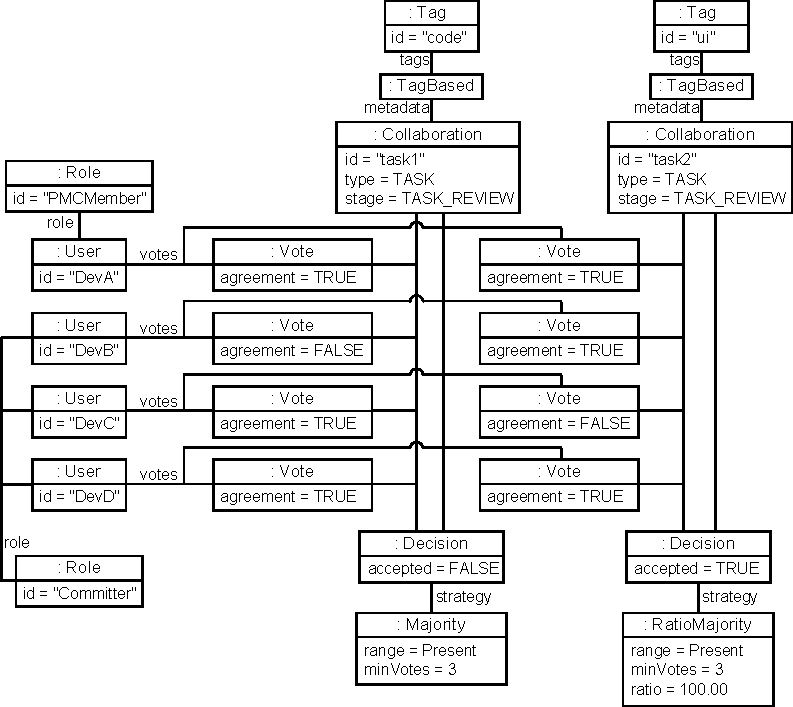
\includegraphics[width=0.65\textwidth]{./figures/exampleCollaborationApache}
  \caption{Example of collaboration in Apache.}
  \label{fig:exampleCollaborationApache}
\end{figure}

%In this section we present an example to illustrate the DSL and the collaboration that may arise. Imagine a development process where the main development tasks are selected according to a democratic process where the developers can participate. The decision process is divided into two phases. During the first phase, the developers team have two hours to vote for/against which existing development tasks should be accomplished, only those ones with a third of simple majority will be selected. In the second phase, those tasks selected in the previous phase are taken into consideration by a committee composed of three senior developers. The committee can must vote for/against the tasks so that only those ones with absolute majority will be selected, in any time the main leader of the team can select the tasks which are urgent, thus avoiding to be voted by yhe senior developers.

%{\footnotesize
%\begin{verbatim}
%Project example {
%  Roles: Developer, Boss, SuperBoss
%  Strategies:
%    myRatioExamples : Ratio {
%      applied to Proposal
%      people Developer
%      range Present
%      minVotes 0
%      ratio 0.66
%    }
%    myMajorityExample : Majority {
%      applied to Proposal
%      people Boss
%      range Present
%      minVotes 0
%    }
%    myPhasedStrategy : Phased {
%      applied to Proposal
%      phases myMajorityExample, 
%             myRatioStrategy
%    }
%}
%\end{verbatim}
%}


%Figure \ref{fig:exampleStrategy} shows the decision strategy model expressed by our DSL for the example. As can be seen, the main decision strategy is a phased strategy (see instance of \texttt{PhasedStrategy} metaclass) composed of two phases. The first phase is an instance of \texttt{RatioMajority} metaclass which considers all the developers as voters, its \texttt{type} attribute is set to \texttt{SIMPLE} to indicate that the majority is simple and its \texttt{ratio} attribute is set to \texttt{0.66} specifying the proportion to fulfill. The deadline for this phase is a \texttt{Timer} instance whose \texttt{mins} attribute is set to \texttt{120} (i.e., two hours). On the other hand, the second phase is an instance of \texttt{LeaderDriven} metaclass which assigns the role of leader to the main team developer (see \texttt{User} metaclass instance with \texttt{id} attribute set to \texttt{SuperBoss}) and its deadline is a \texttt{WaitUserVote} to indicate that the strategy has to wait for the vote of the leader. The default behavior for this strategy is referring to an instance of \texttt{Majority} metaclass with its \texttt{type} attribute set to \texttt{ABSOLUTE} to indicate that the majority is absolute and the users involved are the three senior developers (see \texttt{User} metaclass instances with \texttt{id} attributes set to \texttt{BossA}, \texttt{BossB} and \texttt{BossC}).

%\begin{figure}[t]
%  \centering
%  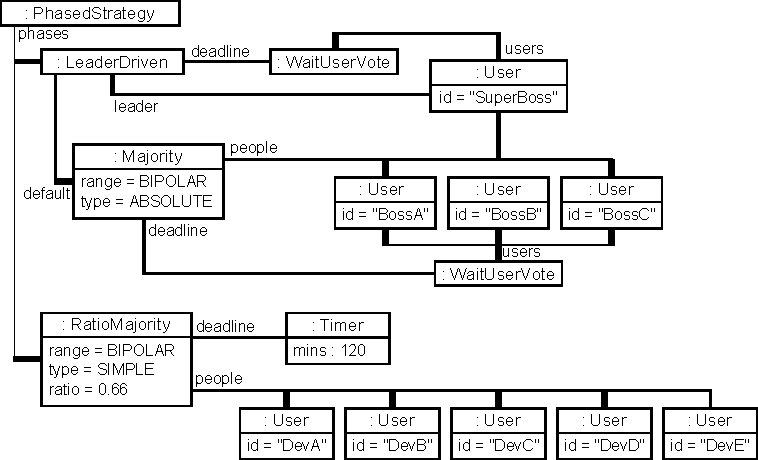
\includegraphics[width=\columnwidth]{./figures/exampleStrategy}
%  \caption{Example of decision strategy}
%  \label{fig:exampleStrategy}
%\end{figure}

%As an example of executing the decision strategy, Figure \ref{fig:exampleCollaboration} shows a possible scenario where team developers have to make a decision about a task proposal with identifier \texttt{task1}. As can be seen, the first phase involves the vote of the developers: users with identifiers \texttt{DevA}, \texttt{Devb} and \texttt{DevC} vote possitively, user with id \texttt{DevD} votes negatively and user with identifier \texttt{DevE} does not vote. The result of the first phase is the aceptance of the proposal to be accomplished so it is then triggered the second phase of the strategy. In the second phase, the leader votes for the proposal so there is on need to make a votation with the senior developers. Thus, the final decision is to accept the proposal.

%\begin{figure}[t]
%  \centering
%  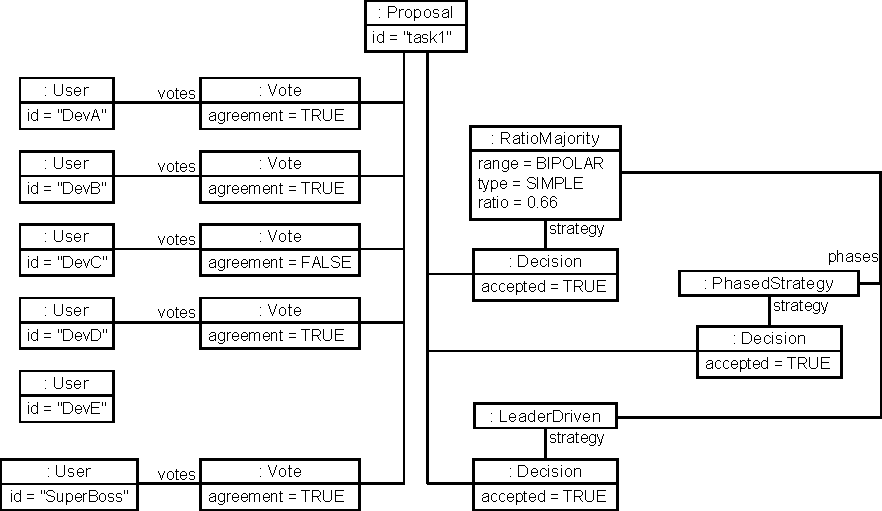
\includegraphics[width=\columnwidth]{./figures/exampleCollaboration}
%  \caption{Example of collaboration}
%  \label{fig:exampleCollaboration}
%\end{figure}



